\documentclass{beamer}
\usetheme{metropolis} % Use the metropolis theme

% Add tikz and pgfplots packages
\usepackage{tikz, pgfplots}
\usetikzlibrary{positioning}

% For clicking references
\usepackage{hyperref}

% For better horizontal lines
\usepackage{booktabs}

% For better referencing
\usepackage{cleveref}

\usepackage{graphicx}


\usepackage{amsmath}

\usepackage{wasysym}

% Define custom pastel colors
\definecolor{pastelRed}{RGB}{255, 105, 97}   % A soft pastel red
\definecolor{pastelBlue}{RGB}{119, 158, 203} % A muted pastel blue
\definecolor{pastelYellow}{RGB}{255, 223, 0} % A gentle pastel yellow
\definecolor{lightGray}{RGB}{211, 211, 211}  % A light gray for subtitles and less emphasized text

% Apply the custom colors
\setbeamercolor{palette primary}{bg=black, fg=white}
\setbeamercolor{palette secondary}{bg=lightGray, fg=black}
\setbeamercolor{palette tertiary}{bg=black, fg=white}
\setbeamercolor{titlelike}{parent=palette primary, fg=black}
\setbeamercolor{subtitle}{fg=lightGray}
\setbeamercolor{structure}{fg=black} % For itemize, enumerate, etc

% Change color of normal text
\setbeamercolor{normal text}{fg=black, bg=white}

% Set the color of the table of contents
\setbeamercolor{section in toc}{fg=black} % Section titles in TOC
\setbeamercolor{subsection in toc}{fg=black} % Subsection titles in TOC

% Set block colors
\setbeamercolor{block title}{use=structure,fg=white,bg=pastelRed}
\setbeamercolor{block body}{fg=black,bg=white}



% Title Page Info
\title{The Min-Cut Problem}
\subtitle{Spørgsmål 10 fra Exam Questions}
\author{Kevin Vinther}
\date{\today}

\begin{document}

% Title Page
\begin{frame}
  \titlepage
\end{frame}

% Table of Contents
\begin{frame}[allowframebreaks]
  \frametitle{Table of Contents}
  \tableofcontents
\end{frame}

\begin{frame}[allowframebreaks]
  \frametitle{The Min-Cut Problem}
  \begin{itemize}
  \item Givet en undirected graf $G = (V,E)$, er et \textit{cut} af $G$ en \textit{partition} af knuder $V$ i to ikke-tomme sæt $A$ og $B$.
  \item Størrelsen af et cut $(A,B)$ er antallet af edges der har start i en partition, og ende i en anden. 
  \item It \textbf{Global Min-cut} er et cut af minimum størrelse
  \item Global betyder at ethvert cut er tilladt, der er ingen source eller sink. 
  \end{itemize}
\end{frame}

\begin{frame}[allowframebreaks]
  \frametitle{Algoritme}
  \begin{theorem}[13.4]
There is a polynomial-time algorithm to find a gloibal min-cut in an undirected graph $G$
  \end{theorem}
  \begin{itemize}
  \item Vi skal først transformere grafen så der er directed kanter, og en \textit{source} og \textit{sink} (genkald flows)
  \item Måden dette bliver gjort på er følgende:
  \item Erstat hver $e = (u,v) \in E$ med $e' = (u,v)$ og $e'' = (v,u)$, hver med en kapacitet af 1. 
  \item Vi kalder den resulterende graf $G'$.
  \item Herefter vælger vi arbitrært to knuder $s, t \in V$
  \item Vi ved at $S$ må være i en af subsetsne, for the sake of example bruger vi $A$. 
  \item Dette betyder at cuttet sepererer $S$ fra alle knuder i $B$. 
  \item VI kan så, for hver knude $\forall t \in V - {s}$ i grafen udregner vi et s-t cut i $G'$. 
  \item Dermed må vi udregne $n-1$ minimum $s-t$ cuts (Siden der er $n$ knuder, og $s$ tæller ikke med.)
  \item Ud af alle disse cuts, vælger vi den der er minimum.
  \item Slut på algoritmen. $\qed$
  \item Trods at det lyder sådan, er denne algoritme meget simpel. Vi bruger Karger's Algoritme som eksempel.
  \end{itemize}
\end{frame}

\begin{frame}[allowframebreaks]
  \frametitle{Karger's Algoritme}
\begin{itemize}
\item Algoritmen, i sin essens, er ikke super optimal. Der er dog blevet lavet optimeringer siden dens fødsel.
\item Algoritmen arbejder på en \textit{connected multigraph} $G = (V,E)$, altså, en undirected graf der tillader flere parallele kanter mellem det samme par af knuder.
\end{itemize}  
\begin{definition}[Muligraph Wikipedia]
A multigraph is a graph which is permitted to have multiple edges, that is, edges that have the same end nodes. Thus two vertices may be connected by more than one edge.
\end{definition}
\begin{itemize}
\item Algoritmen starter med at vælge en kant $e = (u,v) \in G$ \textit{uniformt tilfældigt} og så \textbf{contracter} den den. 
\end{itemize}
\begin{center}
    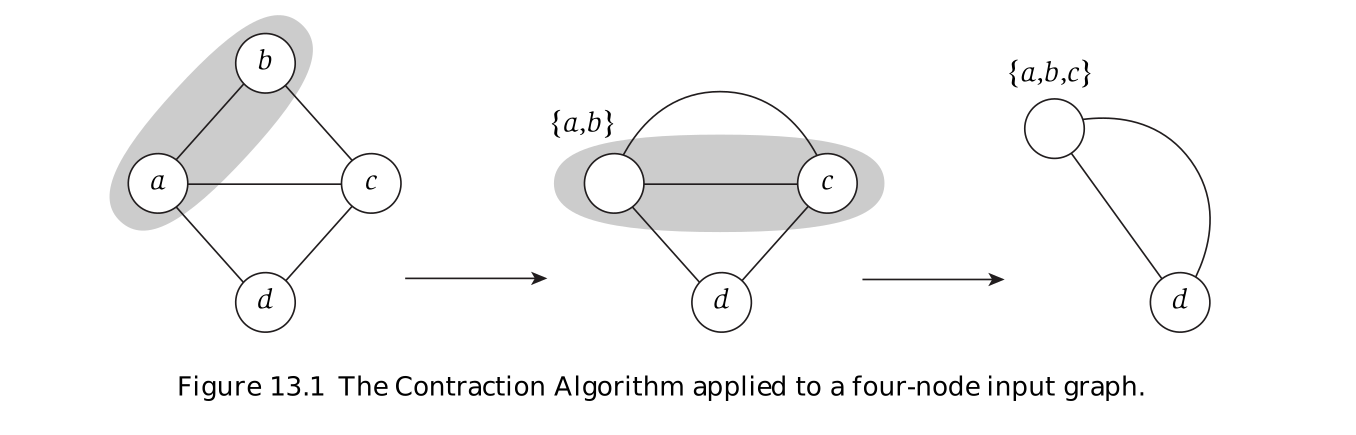
\includegraphics[width=300pt]{main-b690.png}
\end{center}
\begin{itemize}
\item Hvad dette betyder, er at der nu er en ny graf, hvori $u$ og $v$ er blevet til en ny knude $w$. Alle andre knuder forbliver sig selv. 
\item Alle kanter hvor $e = (u,v)$ fjernes, alle andre forbliver.
\item Algoritmen kører så rekursivt på $G'$, og bliver ved med at vælge en kant tilfældigt. 
\item Som disse rekursive kald fortsætter, er de konsttituerende knuder set som \textbf{superknuder}, hver superknude $w$ er $S(w) \subseteq V$ som er blevet ``slugt'' og har produceret $w$. 
\item Algoritmen terminerer når den når en graf med to supernoder $v_{1}$ og $v_{2}$ (sandsynligvis med en masse parallele kanter immelem sig).
\item Hver af disse super-noder $v_{i}$ har en korresponderende subset $S(v_{i}) \subseteq V$, konsisternde af knuder som er blevet contracted ind i sig, og disse to sæt $S(v_{1})$ og $S(v_{2})$ returnerer vi så som svar i form af par. 
\end{itemize}
\begin{center}
    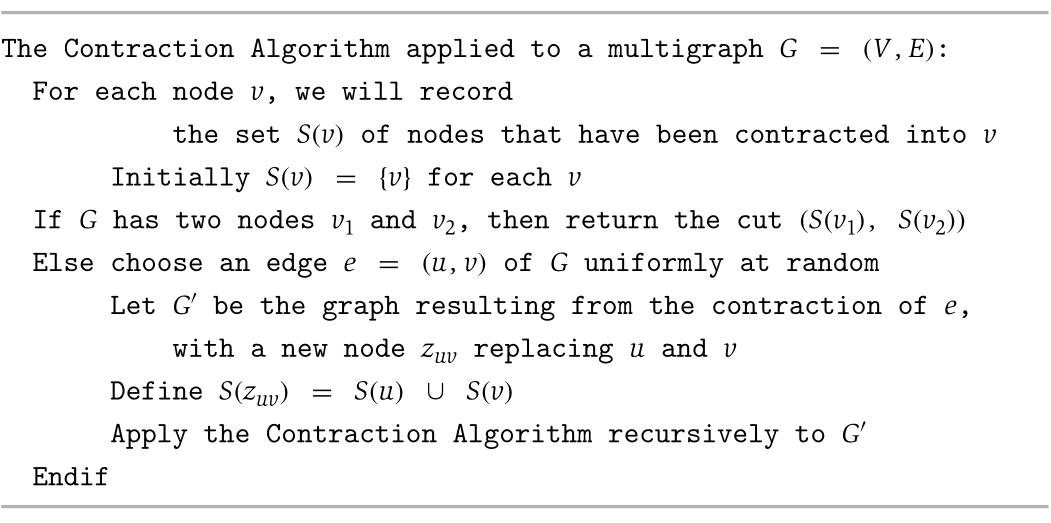
\includegraphics[width=300pt]{main-6240.png}
\end{center}
\end{frame}

\begin{frame}[allowframebreaks]
  \frametitle{Analyse af algoritmen}
 \begin{theorem}
The Contraction Algorithm (Karger) returns a global min-cut of $G$ with probability at least $\frac{1}{\binom{n}{2}}$
 \end{theorem} 
 \begin{itemize}
 \item Vi fokuserer på et globalt min-cut $(A,B)$ af $G$. 
 \item Vi antager at det (i.e. cuttet) tager størrelsen $k$. 
 \item Altså: der er et sæt $F$ af $k$ kanter, med en ende i $A$ og en anden i $B$
 \item Vores mål er at finde et lower bound. 
 \item Muligt problem: Hvis en kant i $F$ bliver contracted, ville en knude fra både $A$ og $B$ blive contracted til en superknude.
 \item Hvis dette sker, kan $(A,B)$ ikke blive returneret som output. 
 \item Omvendt, hvis $E \notin F$ bliver contracted, er der en mulighed for at $(A,B)$ bliver returneret. 
 \item Vi vil gerne finder et upper bound på sandsynligheden at en kant i $F$ bliver contracted. 
 \item For at kunne finde denne upper bound, skal vi bruge en lower bound på størrelsen af $E$ (antal kanter).
 \item Antag at en knude $v$ har \textit{degree} (antal kanter) mindre end $k$ (antal kanter mellem A og B). 
 \item Så er cuttet $(\{v\}, V - \{v\})$ af størrelse mindre end $k$, som er imod vores antagelse at $(A,B)$ er global min-cut. (Fordi den er for lille)
 \item Derfor har enhver knude i $G$ en degree af \textbf{mindst} $k$. Dermed $|E| \geq \frac{1}{2}kn$ hvor $n$ er antal knuder. $\frac{1}{2}kn$ kommer fra en kant per knude. Dermed $\frac{1}{2}k$ i stedet for bare $kn$  (i.e., der kan mindst være én kant fra knude til knude.)
 \item Dermed er sandsynligheden at en kant i $F$ bliver contracted højest \[ \frac{k}{\frac{1}{2}kn} = \frac{2}{n}  \]
 \item Fordi der er $k$ af disse edges, så det er $k$ mulige ud af upper bound $|E| = \frac{1}{2}kn$ (Den her bog gør det meget sværere end det behøver at være)
 \item Lad os nu kigger på situationen efter $j$ iterationer, når der er $n-j$ superknuder i vores nuværende graf $G'$ og antag at ingen kant i $F$ er blevet contracted endnu.
 \item Så bliver udregningen \[ \frac{k}{\frac{1}{2}k(n-j)} = \frac{2}{n-j} \]
 \item Vi ved at cuttet $(A,B)$ vil blive returneret hvis ingen kant i $F$ bliver contrracted i iterationerne $a,2, \ldots, n-2$. 
 \item Lad $\varepsilon_{j}$ være hændelsen at en kant af $F$ \textbf{ikke} bliver contracted  i iteration $j$, så har vi vist at $P(\varepsilon_{j}) \geq 1 - \frac{2}{n}$ og at $P(\varepsilon_{j+1} | \varepsilon_{1} \cap \cdots \cap \varepsilon_{j}) \geq 1 - \frac{2}{n-j}$.
 \item Nu vil vi gerne finde en lower-bound på $P(\varepsilon_{1} \cap \cdots \cap \varepsilon_{n-2})$.
 \end{itemize}

 \begin{equation}
\begin{split}
  P(\varepsilon_{1}) &\cdot P(\varepsilon_{2}| \varepsilon_{1}) \cdots P(\varepsilon_{j+1} | \varepsilon_{1} \cap \varepsilon_{2} \cap \cdots \cap \varepsilon_{j}) \cdots P(\varepsilon_{n-2} | \varepsilon_{1} \cap \cdots \cap \varepsilon_{n-2})\\
           &\geq \left( 1- \frac{2}{n} \right) \left( 1-\frac{2}{n-1} \right) \cdots \left( 1 - \frac{2}{n-j} \right) \cdots \left( 1 - \frac{2}{3} \right)\\
           &= \left( \frac{n-2}{n} \right) \left(  \frac{n-3}{n-1} \right) \left( \frac{n-4}{n-2} \right) \cdots \left( \frac{2}{4} \right) \left( \frac{1}{3} \right)\\
  &= \frac{2}{n(n-1)} = \binom{n}{2}^{-1}. \qed
\end{split}
 \end{equation}

\begin{itemize}
\item Vi ved nu at et enkelt \textit{run} af Kargers Algoritme fejler med sandsynligheden $1- \frac{1}{\binom{n}{2}}$ (dette er et tal der er meget tæt på 1).
\item $1 - \frac{1}{\binom{5}{2}} = 90\%$
\item $1 - \frac{1}{\binom{50}{2}} = 99.9\%$
\item $1 - \frac{1}{\binom{500}{2}} = 99.999\%$
\item $1 - \frac{1}{\binom{5000}{2}} = 99.999999\%$
\item Vi kan dog få sandsynligheden til at blive lidt bedre ved at køre algoritmen igen og igen og ved brug af tilfældige valg. 
\item Vi ved fra kapitel 1 at hvis vi kører algoritmen $\binom{n}{2}$ gange, så er sandsynligheden:
\[ \left( 1- \frac{1}{\binom{n}{2}} \right)^{\binom{n}{2}}  \leq \frac{1}{e}\]
\end{itemize}

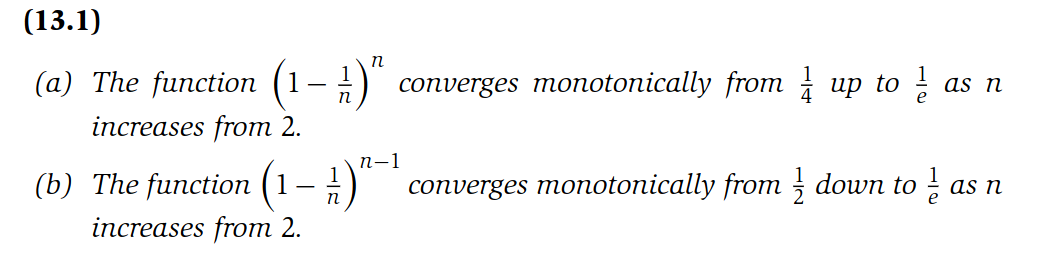
\includegraphics[width=300pt]{main-ab7f.png}

\begin{itemize}
\item Vi kan gå endnu lavere. Hvis vi kører algoritmen $\binom{n}{2} \ln n$ gange, så er sandsynligheden for at vi fejler i at finde et global min-cut \textbf{højest} $e^{-\ln n} = 1/n$. (Jeg er ikke helt sikker på hvorfor?)
\end{itemize}
 

\begin{theorem}[13.6]
An undirected graph $G = (V,E)$ on $n$ nodes has at most $\binom{n}{2}$ global min-cuts.
\end{theorem}
\begin{itemize}
\item Lad $G$ være en graf, og lad $C_{1}, \ldots, C_{r}$ være alle dets global min-cuts. 
\item Lad $\varepsilon_{1}$ være hændelsen at $C_{i}$ er returneret af Contraction Algoritmen, og lad $\varepsilon = \bigcup^{r}_{i=1}\varepsilon_{i}$ være hændelsen at algoritmen returnerer et min-cut.
\item Vi ved fra 13.5 at $P(\varepsilon) \geq \frac{1}{\binom{n}{2}}$.
\item Faktisk viser beviset at for hvert $i$ har vi $P(\varepsilon_{i}) \geq \frac{1}{\binom{n}{2}}$. 
\item Hver par af hændelser $\varepsilon_{i}$ og $\varepsilon_{j}$ er disjunkte, dermed ved vi fra union bound at:
  \[  P(\varepsilon) = P(\bigcup\limits_{i=1}^{r} \varepsilon_{i}) = \sum_{i=1}^{r}P(\varepsilon_{i}) \geq \frac{r}{\binom{n}{2}} \]
  \item Ud fra dette kan vi så tydeligt se at $r \leq \binom{n}{2}$.
\end{itemize}
\end{frame}

\begin{frame}[allowframebreaks]
  \frametitle{Max-back orderings}
  \begin{itemize}
  \item 10 sider :(
  \item Givet en undirected multigraf $G = (V,E)$, kan edge-connectivitiy $\lambda(G)$ blive fundet ved brug af $n-1$ max-flow udregninger. 
  \end{itemize}
  \begin{definition}[Edge-Connectivity]
The edge connectivity, also called the line connectivity, of a graph is the minimum number of edges whose deletion from a graph disconnects. In other words, it is the size of a minimum edge cut. (Kilde: Wolfram MathWorld)
  \end{definition}
  \begin{itemize}
  \item Vi starter ud med nogle lemmaer og definitioner
  \end{itemize}
  \begin{definition}[1 (Max-back Ordering)]
    A max-back ordering of a given undirected multigraph $G$ is an ordering $v_{1}, v_{2}, \ldots, v_{n}$ of the vertices of $G$, satisfying the inequality
    \[ d(V_{i}, v_{i+1}) \geq d(V_{i}, v_{j}) \]
    for all indices $i$ and $j$,$1 \leq i < j \leq n$. The set $V_{i}$ is defined by $V_{i} = \{v_{1}, v_{2}, \ldots, v_{i}\}$.
  \end{definition}
  \begin{itemize}
  \item Ifølge ChatGPT betyder $d$ sandsynligvis antallet af degrees.
  \end{itemize}
  \begin{lemma}[1]
A max-back ordering of a given undirected multigraph $G = (V,E)$ can be found in $O(|V| \log |V| + |E'|)$ time, where $E'$ is the set of edges in the corresponding simple graph.
  \end{lemma}
\end{frame}

\end{document}